%This file will be included in the ThesisMain Document as the Experimental
%apparatus section section.

%Author: James Kelly
%Last Modified: 10-08-08

\doublespacing
\begin{center}
\section{INTRODUCTION}
\end{center}

\pagenumbering{arabic}
\subsection{Overview}
Physiographic regions are generalized as mountainous or upland based on three outstanding geological characteristics: Steep slopes, large relief and elevated bedrock. In contrast to neighboring lowland or piedmont regions, upland regions demonstrate a different set of geological behaviors, across all scales of observation. Consequently upland watersheds are decidedly unique due to their geographical location, and directly as a result of these upland characteristics, they are more sensitive to their inputs \citep{watersheds}.

Currently, urban and suburban development pervades upland regions worldwide at ever increasing rates and densities \citep{rgis}. Specific findings on upland ecological systems and overall watershed health are emerging to show developmental management practices that may be well suited for lowland regions are not effective, or perhaps more hurtful, in upland regions \citep{urban}. It is the intent of this research to further contribute to this emerging understanding regarding upland ecology, geology and impact assessment.

The research and experiments presented in this thesis were further motivated from the realization that some best management practices (BMP) and other common engineering solutions to watershed management may be ornamental, and poorly suited for an upland context \citep{urban}. Specifically, we focused on the use of construction aggregate and other unconsolidated material to thermally sink stormwater discharge at point sources. It is a common practice to fill an entrenchment intended for infiltration or local discharge with gravel, especially near waters that are sensitive to thermal charging \citep{rgis}. The gravel provides armament for the entrenchment and also is figured to thermally sink the effluent before being discharged \citep{ballast}. The discharge or surface flow interacts with the gravel in a complex and variable manner that would be difficult to measure or characterize. However, an understanding of the amount of a particular mass of aggregate could ideally sink and the rate at which the heat could be transferred could potentially offer motivations for additional solutions of thermal mitigtion or at least offer insight into the current arrangements of entrenched gravel and stream bank stabilization techniques \citep{kRocks}.

\subsection{Upland Watershed Characteristics}
Watersheds that drain upland regions are consistently dendric, high gradient waters. Using hydrogeologic definitions of order 1 being an intermittent drainage and order 5 being a large, high volume, mature river, most mountain reaches are of order 2 or less, with some prominent drainages no higher than grade 3 \citep{watersheds}. The streambeds are composed of large grains and cobbles due to intermittently large flow volumes with very high flow energies, steep profiles and elevated rates of bank erosion \citep{thaxAdd}. Due to characteristically thin soil horizons, infiltration in catchment areas is notoriously shallow, which limits baseflow causing many upper reaches to be highly intermittent, fast draining and excessively “flashy” \citep{krautBASE}. Upland waters are comparably cold, oxygen rich waters that foster a seperate ecology from lowland regions. Regional biota are, to  some degree, acclimated to frequent changes in volume and sediment load, but remain highly susceptable to large changes in water temperture \citep{urban}. Stream temperature in general serves as an excellent indicator of many upland freshwater ecosystems, because the populations are so temperature dependent. These upland waters are more sensitive to thermal inputs from all sources, such baseflow, surface heating and discharges \citep{anderson}. 

\subsection{Summary of Impacts}
Urban and suburban development fundamentally impacts these waters through variances in surface and baseflow volumes, extreme sediment loading and thermal charging, not to mention other types of explicit pollution \citep{rgis}. The sometimes shallow infilitration, and generally small aquifer size and faster baseflows that define upland hydrology are dramatically effected by dense urban development. Urban surfaces such as rooftops, streets, sidewalks and parking lots further prevent infiltration and rapidly evacuate stormwater into the nearest surface flow \citep{rgis, krautBASE}. Additionally, the installation of culverts to control flow and channelization eliminate groundwater interaction \citep{anderson}. Thermal charging occurs primarily as a result of point sources from either urban surfaces as stormwater discharge, from retention pond overflow or from industrial discharges \citep{krautBASE}.

\subsection{Boone Creek Monitoring}
Stream data are currently being collected on the Appalachian State University campus in and around Boone Creek. Boone Creek is a first-order tributary of the New River, a National Heritage River. It is typical of an upland creek, exhibiting frequent high-energy flows, a course grain streambed, rapid draining of its catchment area and, consequently, susceptibility to flash floooding. As is common with upland watersheds, the Boone Creek area is subjected to seasonal orographic storms of near daily frequency during the spring and summer months. Thermal spikes in the creek flow on the order of $2-6^{o}$ C have been measured during these warmer months, indicative of urban thermal charging. \linebreak Figure (\ref{kcPeak}) features data that illustrate a thermal spike at three stream locations during a rain event on June 23, 2006.

\begin{figure}[h!]
\begin{center}
 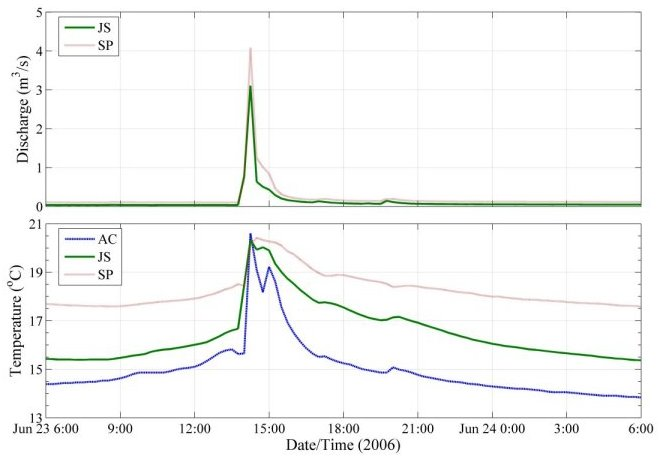
\includegraphics[scale=0.7]{kc_peak.jpg}
\caption[Boone Creek Thermal Charging]{\textbf{\emph{Thermal Charging During Stream Peakflow}} Stream temperature as measured in the highly urbanized Boone Creek during peak stream flow from a storm. Agricultural Center (AC), Jimmy Smith Park (JS) and Steam Plant (SP) indicate measurement positions in a downstream order. The top plot illustrates a spike in steamflow, and the lower plot shows a corresponding spike in stream temperature as a result of some thermally charged point source(s) emptying into the creek. The exact sources for this thermal charging are currently being researched and could include pond overrun or heat from urban surfaces \citep{krautBASE}.\label{kcPeak}}
\end{center}
\end{figure}

These temperature spikes coincide with the onset of sudden afternoon storms that have the capacity for high precipitation rates. This is coupled with the intense heating of urban surfaces that often precedes the afternoon storms. The stormwater channelization from urban surfaces into the surface flow offers virtually no deliberate mechanism for thermal buffering in the current infrastructure regime, and the high precipitation rate ensures that this thermal energy is efficiently evacuated from the surfaces. Additionally, ther thermal charging data presented in Figure (\ref{kcPeak}) supports the hypothesis that shallow retention pond overflow provides a potent point source for themal charging and are not effective best mangement practices (BMP) in their own right \citep{thaxAdd2}. Not only is the retention pond caching solar energy more efficiently than an urban surface during the heating of the day, but it will also receive the potentially hot flash flow from its own catchment.

\subsection{Thermal Remediation Practices}
Current findings and attitudes toward stream restoration agree that the fundamental goal of any restoration effort is to minimize human imposed change on the physical and biological characteristics of a watershed \citep{watersheds,urban}. This does not mean eliminating human activity or impact on the watershed, but instead approaching restoration as a process of mitigating and managing these impacts through well researched methods \citep{rgis}. In the context of thermal remediation, the ideal solutions would involve shade and infiltration. Realistically, dense urban development sheds volumes of stormwater that is obviously proportional to the precipitation, and this is inevitably accumulated, collected and discharged, directly impacting the volume and rate of return in watershed surface and baseflow. The infrastructure pathways that manage this discharge are typically point source outlets in the form of a pipe that releases the stormwater directly into a creek or retention pond. 

Thermally buffering this discharge presents a difficult engineering problem, especially in the situation of upland topography. In upland development real estate is available only at a premium due to the more severe topographical conditions that restrict how and where any sort of development may occur. Sufficiently large retention basins, infiltration zones and even shade are often not practical provisions that accompany dense urban or suburban development in any sort of region, let alone the space-confined upland regions. End-of-pipe and other confined space solutions offer some potential to buffer an initial thermal charge that may accompany a sudden stormwater flush. As shown below, the quantity of aggregate is still significant, and any doctrine for effective thermal buffering would be centered around removing small amounts of heat energy in enumerable locations with small aggregate masses, as opposed to a few large entrenchments with large masses of material. The material does not need to remove all heat energy, but collectively it should exhibit a reasonably large thermal conductivity and specific heat such that the spike of any thermal charge is damped. Optimizing the geometry of aggregate arrangement, type or size of aggregate cobble and maximizing the contact area with discharge flow would be paramount in implementing any sort of solution. 

\subsection{Using Construction Aggregate for Thermal Mitigation}
The focus on construction aggregate is one that stems primarily from a cost to benefit reality, availability and ease of implementation \citep{ballast}. Although it may not be the optimal material, developers have easy access to it and it is affordable. It can readily be installed with minimal effort, although routine maintenance may be required.
 
Construction aggregate is typically available as a regional product. This causes the material of the aggregate to vary considerably which will effect heat capacities, exchange rates and to a lesser degree, flow capacity. Local quarries usually produce a range of cobble sizes, ranging from 3/8'' to 4'' in mean diameter, or more formally measured on site with a series of sieves to rate a particular sample with a fineness modulus. Geometry of the cobbles is always irregular, with some rock types yielding a flatter “chip” type of cobble, which stands to lower the compaction and bulk porosity of the aggregate, at the same time increasing its bulk density. 


